\chapter{Cơ sở lý thuyết liên quan đề tài nghiên cứu}

\section{Giới thiệu hệ thống robot thực nghiệm}
\begin{figure}[tph]
	\centering
	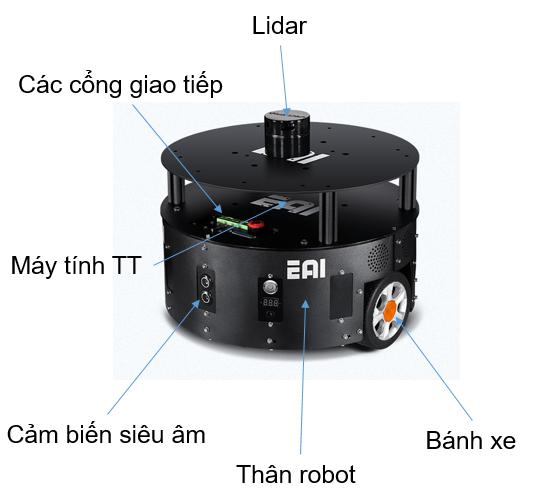
\includegraphics[width=0.7\linewidth]{chapter1/figs/eaiD1}
	\caption{Cấu tạo robot}
	\label{fig:eaid1}
\end{figure}

Toàn bộ nghiên cứu về các giải thuật điều khiển robot sẽ được ứng dụng trên mô hình robot di động thật như trong \figurename{\ref{fig:eaid1}}. 

Đây là một nền tảng robot di động, có cấu tạo:
\begin{itemize}
	\item Hệ thống di chuyển: 2 bánh xe chủ động và 2 bánh xe bị động. 
	\item Cảm biến: Được trang bị 3 cảm biến sonar ở phía trước. Cảm biến Lidar 360 độ được gắn ở trên đỉnh robot.
	\item Bộ điều khiển trung tâm là một máy tính nhúng mini Raspberry Pi 3, chạy hệ điều hành Raspbian	
\end{itemize}

Đây là nền tảng robot tự hành đã được nhà cung cấp phát triển mã nguồn mở các gói lệnh trong ROS, bao gồm các chức năng cơ bảntạo bản đồ môi trường, di chuyển tới vị trí xác định, tránh vật cản trong quá trình di chuyển...


\section{Tổng quan về hệ điều hành ROS}
\textbf{Robot Operating System (ROS)} là một mã nguồn mở, là hệ điều hành cho robot. Nó cung cấp các dịch vụ mà bạn sẽ mong muốn từ một hệ điều hành, cài đặt các hàm được dùng chung, trao đổi thông điệp giữa các tiến trình, và quản lý các gói lệnh. Nó cũng cung cấp các công cụ và các thư viện để lập trình, chạy các nút thông qua nhiều máy tính khác nhau. 

Theo một cách khác, ROS bao gồm các lớp mô tả phần cứng tương tự như hệ điều hành. Tuy nhiên, không giống như các hệ điều hành thông thường, nó có thể được dùng để tích hợp rất nhiều phần cứng với nhau. Hơn nữa, đây là nền tảng phần mềm robot cung cấp rất nhiều môi trường phát triển cho việc phát triển các chương trình ứng dụng robot.

Nói một cách dễ hiểu, theo tác giả, ROS là một nền tảng cung cấp các phương thức để kết nối, trao đổi dữ liệu, quan sát dữ liệu giữa rất nhiều phần cứng với nhau như các cảm biến, các bộ phận chấp hành và các máy tính. Khi sử dụng ROS, người phát triển robot không cần quan tâm quá nhiều đến các thiết bị phần cứng (nếu thiết bị đó đã có thư viện driver ROS hỗ trợ), chỉ cần quan tâm đên việc tính toán, xử lý các dữ liệu để đạt được các mục đích trong các ứng dụng khác nhau. Nó làm giảm thời gian, giảm độ phức tạp khi phát triển robot đi rất nhiều lần. 

Vậy có phải ROS là một hệ điều hành mới, dành riêng cho robot?

ROS là viết tắt của cụm từ Robot Operating System, cũng được dịch ra là Hệ điều hành robot. Tuy nhiên, chính xác hơn thì ROS là một Meta-Operating System. Mặc dù cụm từ Meta-Operating System không được định nghĩa trong từ điển (có thể tạm dịch là Hệ điều hành biến đổi) , nó mô tả một hệ thống thực hiện các quá trình như lập lịch, nạp tải, giám sát và kiểm soát lỗi bằng lớp ảo hóa giữa các ứng dụng và phân tán nguồn lực tính toán.

Tuy nhiên, ROS không phải là hệ điều hành thông thường như như Window, Linux hay Android, nhưng một Hệ điều hành biến đổi chạy trên các nền tảng hệ điều hành có sẵn khác. Để chạy ROS thì phải cài đặt trước hệ điều hành như Ubuntu (một bản phát hành của Linux). Sau khi hoàn thành cài đặt ROS trên nền Ubuntu,  các tính năng từ hệ điều hành như hệ thống quản lý quá trình, hệ thống tệp tin, giao diện người dùng và các chương trình tiện ích khác vẫn có thể sử dụng. Thêm vào đó, ROS cung cấp các hàm cần thiết cho lập trình robot, các thư viện như: truyền/nhận dữ liệu giữa các phần cứng, lập lịch, kiểm soát lỗi. Dạng phần mềm này cũng có thể dược gọi là phần sụn hoặc khung phần mềm.

\begin{figure}[htp]
	\centering
	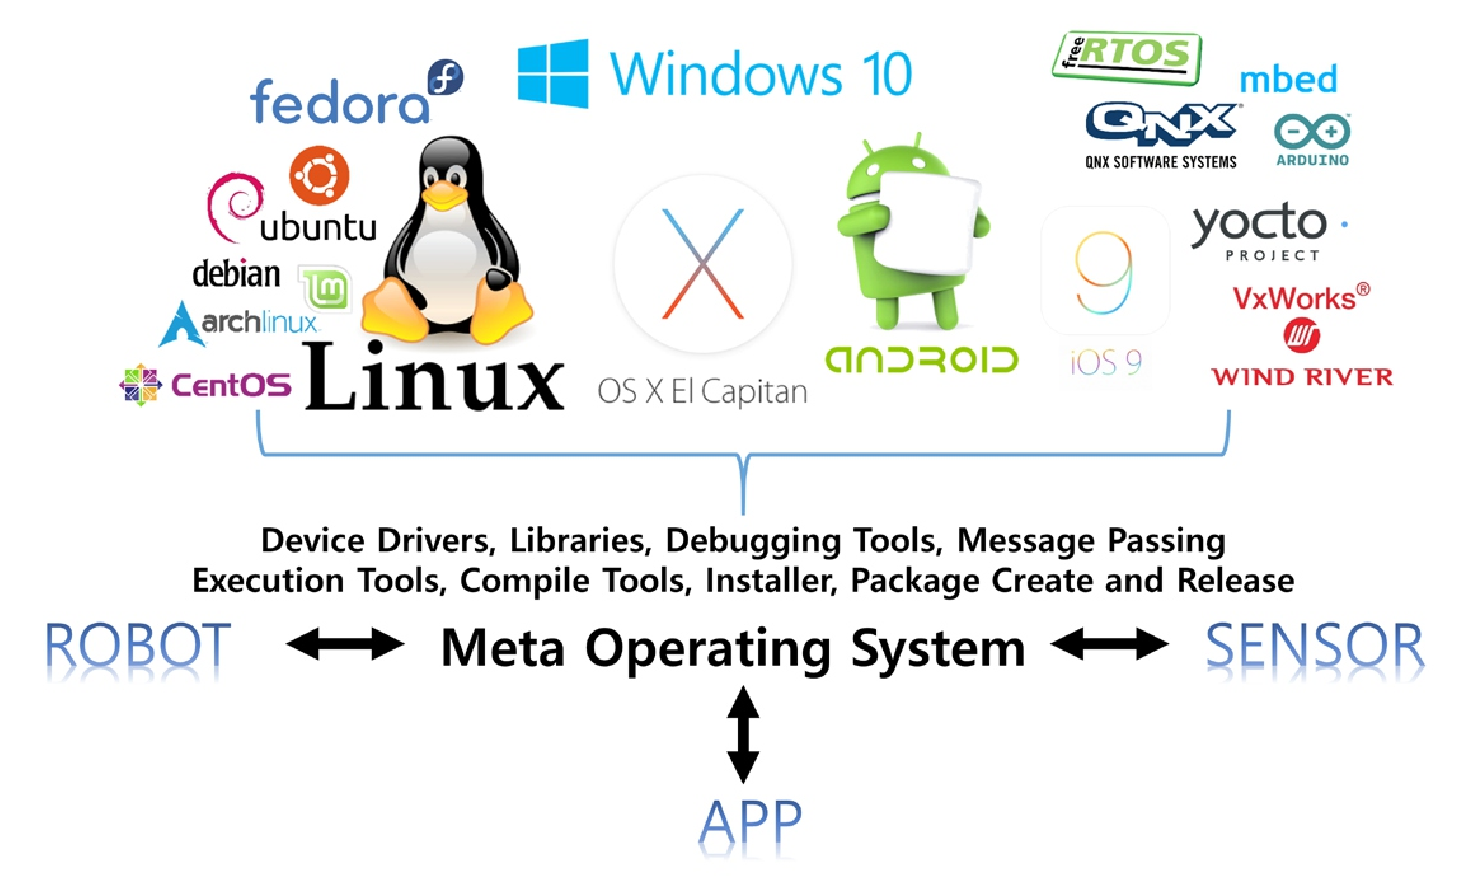
\includegraphics[width=1\linewidth]{chapter2/figs/meta_operatingSystem.pdf}
	\caption{ROS như một Meta-Operating System}
	\label{fig:ROSasMetaOS}
\end{figure}

Như một Hệ điều hành biến đổi, ROS được phát triển, quản lý, cung cấp các gói thư viện ứng dụng cho rất nhiều mục đích và nó có dạng một hệ sinh thái, phân phối các gói thư viện được phát triển bởi người dùng. Như mô tả ở \figurename{\ref{fig:ROSasMetaOS}}, ROS là một hệ thống hỗ trợ cho việc điều khiển một robot và cảm biến với một sự trừu tượng hóa phần cứng và việc phát triển ứng dụng robot dựa trên các hệ điều hành thông thường.

\begin{figure}[htp]
	\centering
	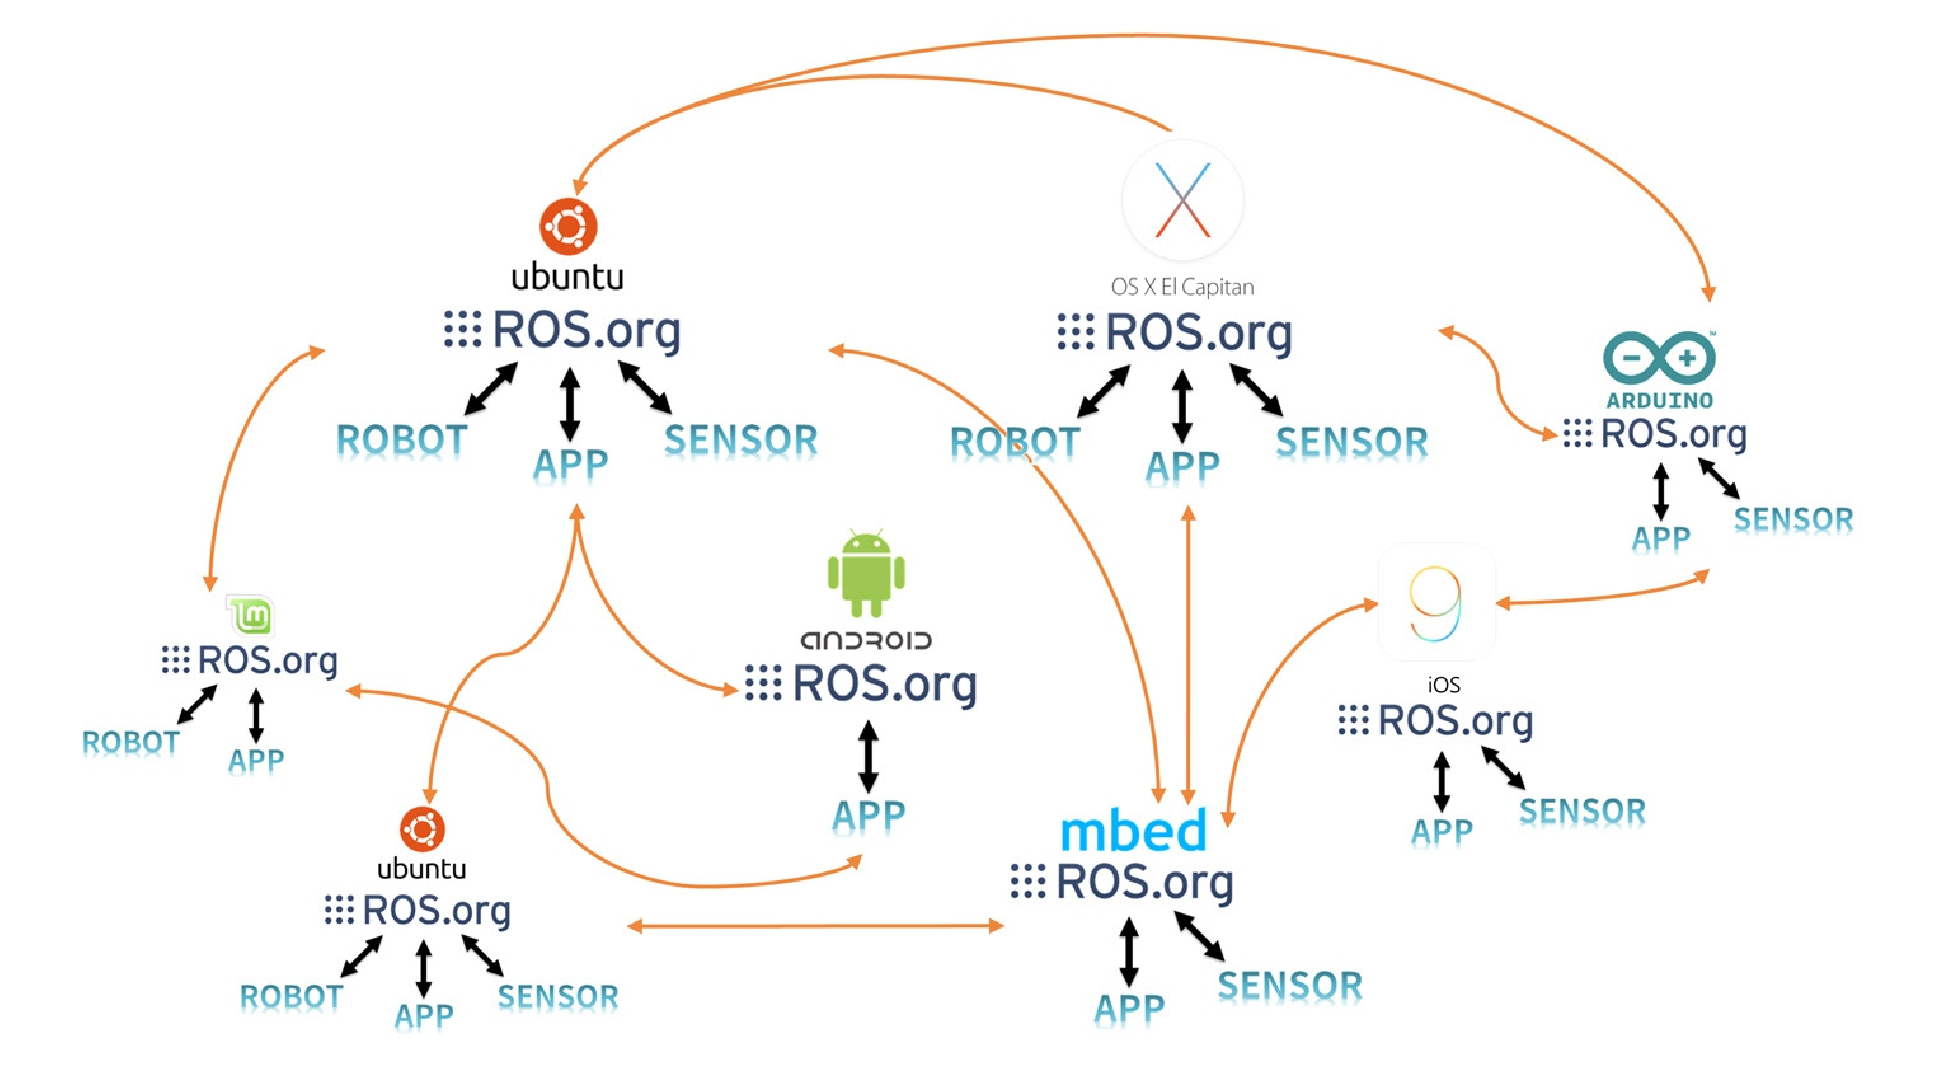
\includegraphics[width=1\linewidth]{chapter2/figs/multi_communication.pdf}
	\caption{Đa giao tiếp trong ROS}
	\label{fig:MultiCommunication}
\end{figure}

Như \figurename{\ref{fig:MultiCommunication}}, giao tiếp dữ liệu ROS được hỗ trợ không chỉ bởi một hệ điều hành, mà bởi nhiều hệ điều hành, phần cứng và chương trình, rất phù hợp cho phát triển robot nơi có rất nhiều phần cứng phối hợp với nhau. 
\cite{Pyo2017}

\begin{figure}[htp]
	\centering
	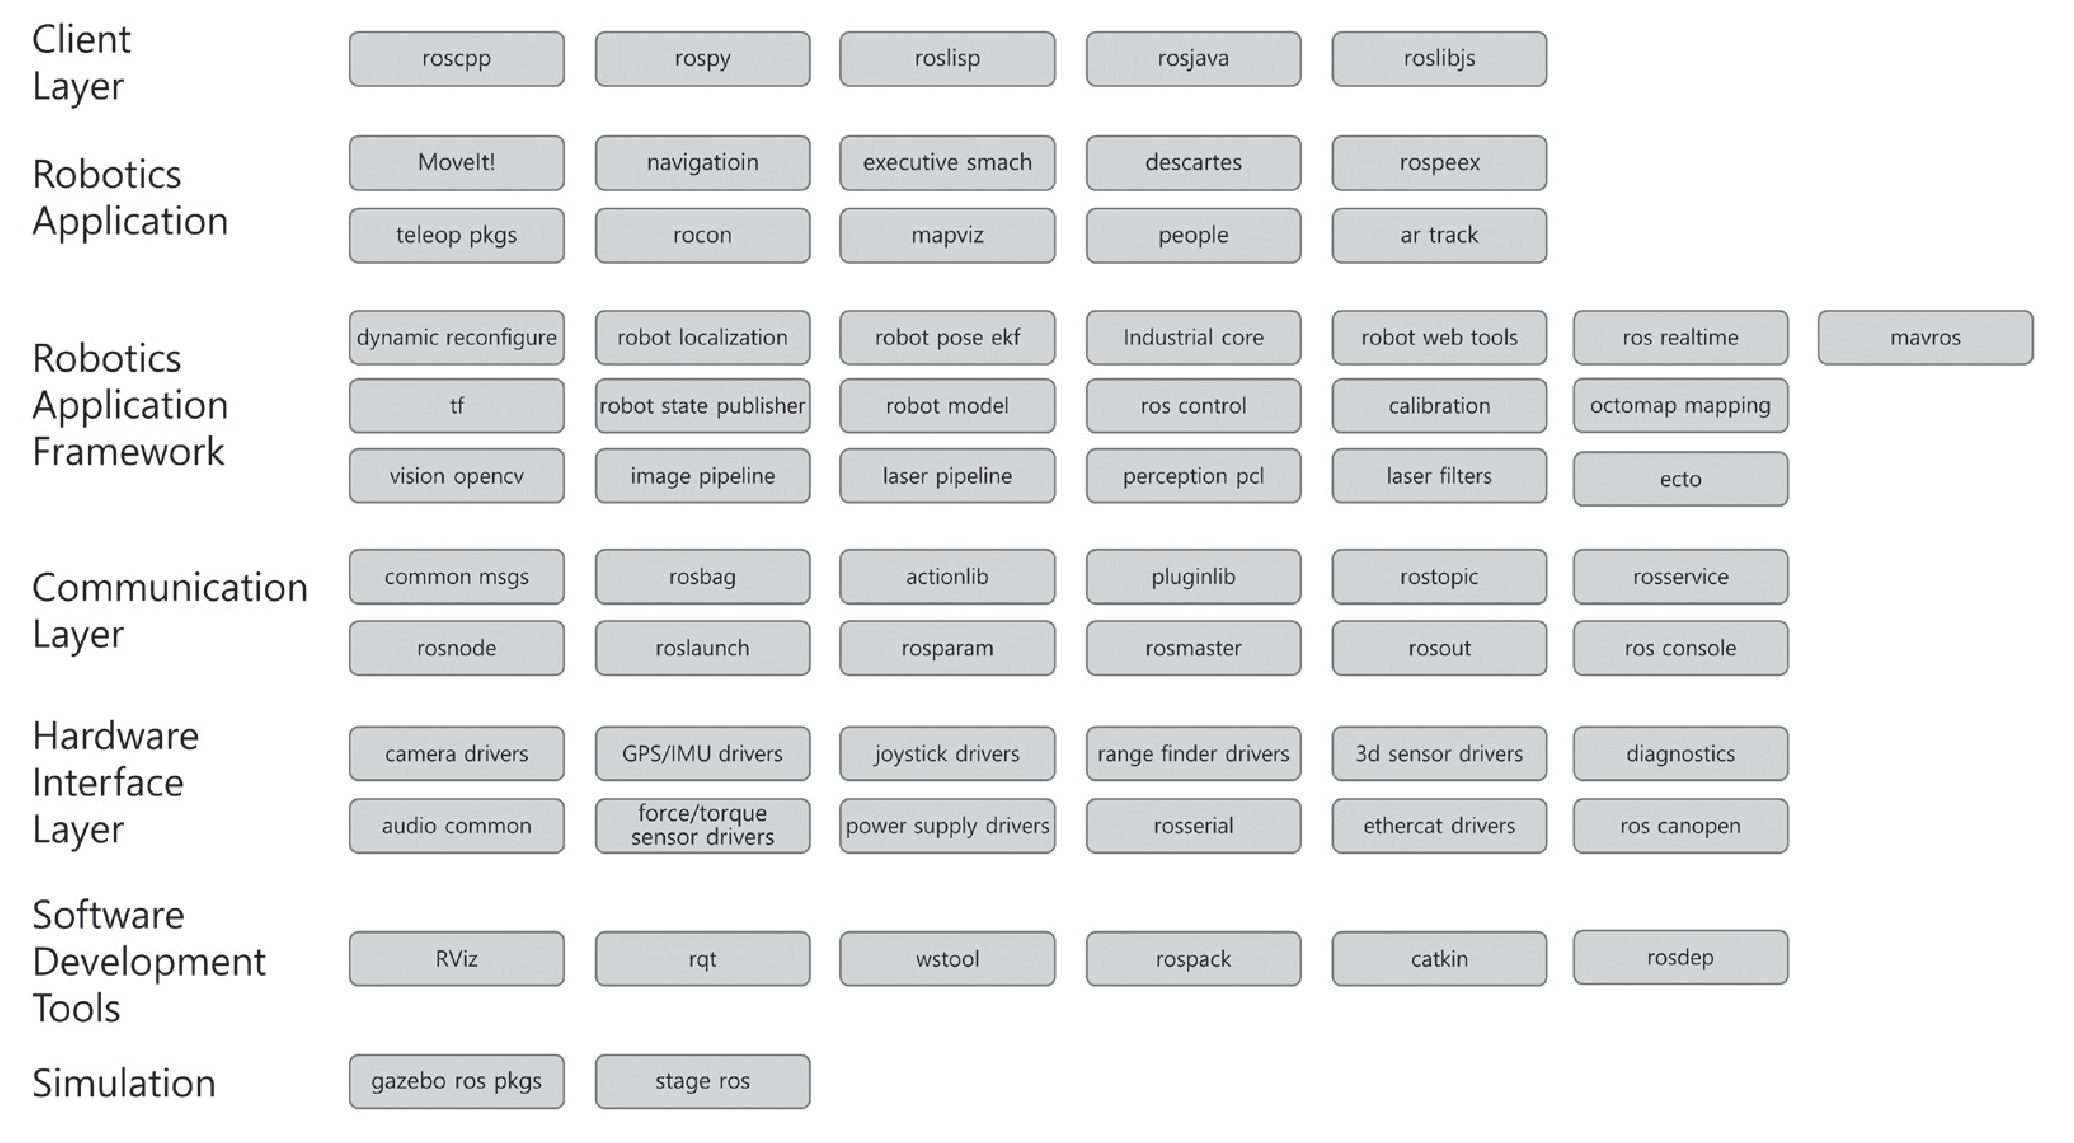
\includegraphics[width=1\linewidth]{chapter2/figs/components.pdf}
	\caption{Các thành phần trong ROS}
	\label{fig:components}
\end{figure}

Như \figurename{\ref{fig:components}}, ROS bao gồm thư viện khách hàng hỗ trợ nhiều ngôn ngữ lập trình khác nhau, một giao tiếp phần cứng cho việc điều khiển phần cứng, giao tiếp cho truyền và nhận dữ liệu, khung ứng dụng robotics giúp tạo ra nhiều ứng dụng robotics, ứng dụng robotics là một ứng dụng dịch vụ dựa trên khung ứng dụng robotics, các công cụ mô phỏng có thể điều khiển robot trong không gian ảo, và các công cụ phát triển phần mềm. 

Cụm từ Hệ sinh thái thường được nhắc đến trên thị trường smartphone sau khi hàng loạt hệ điều hành ra đời như Android, iOS, Symbian... Hệ sinh thái nhắc đến cấu trúc liên kết giữa nhà sản xuất phần cứng, công ty phát triển hệ điều hành, nhà phát triển ứng dụng và người dùng đầu cuối.

Ở đây, robotics cũng có dạng như một hệ sinh thái. Có rất nhiều thiết bị phần cứng được sản xuất và ngày càng phát triển nhiều hơn nữa, nhưng không có một hệ điều hành để tích hợp chúng. Một vài nền tảng phần mềm xuất hiện và ROS thu hút được đủ sự chú ý để xây dựng một hệ sinh thái. Mặc dù tác động của nó chưa đủ lớn, nhưng với sự gia tăng của số lượng người dùng, các công ty liên quan đến robot, các thư viện, công cụ liên quan, chúng ta có thể thấy được một hệ sinh thái đầy đủ các chức năng trong tương lai gần. 
\begin{figure}[htp]
	\centering
	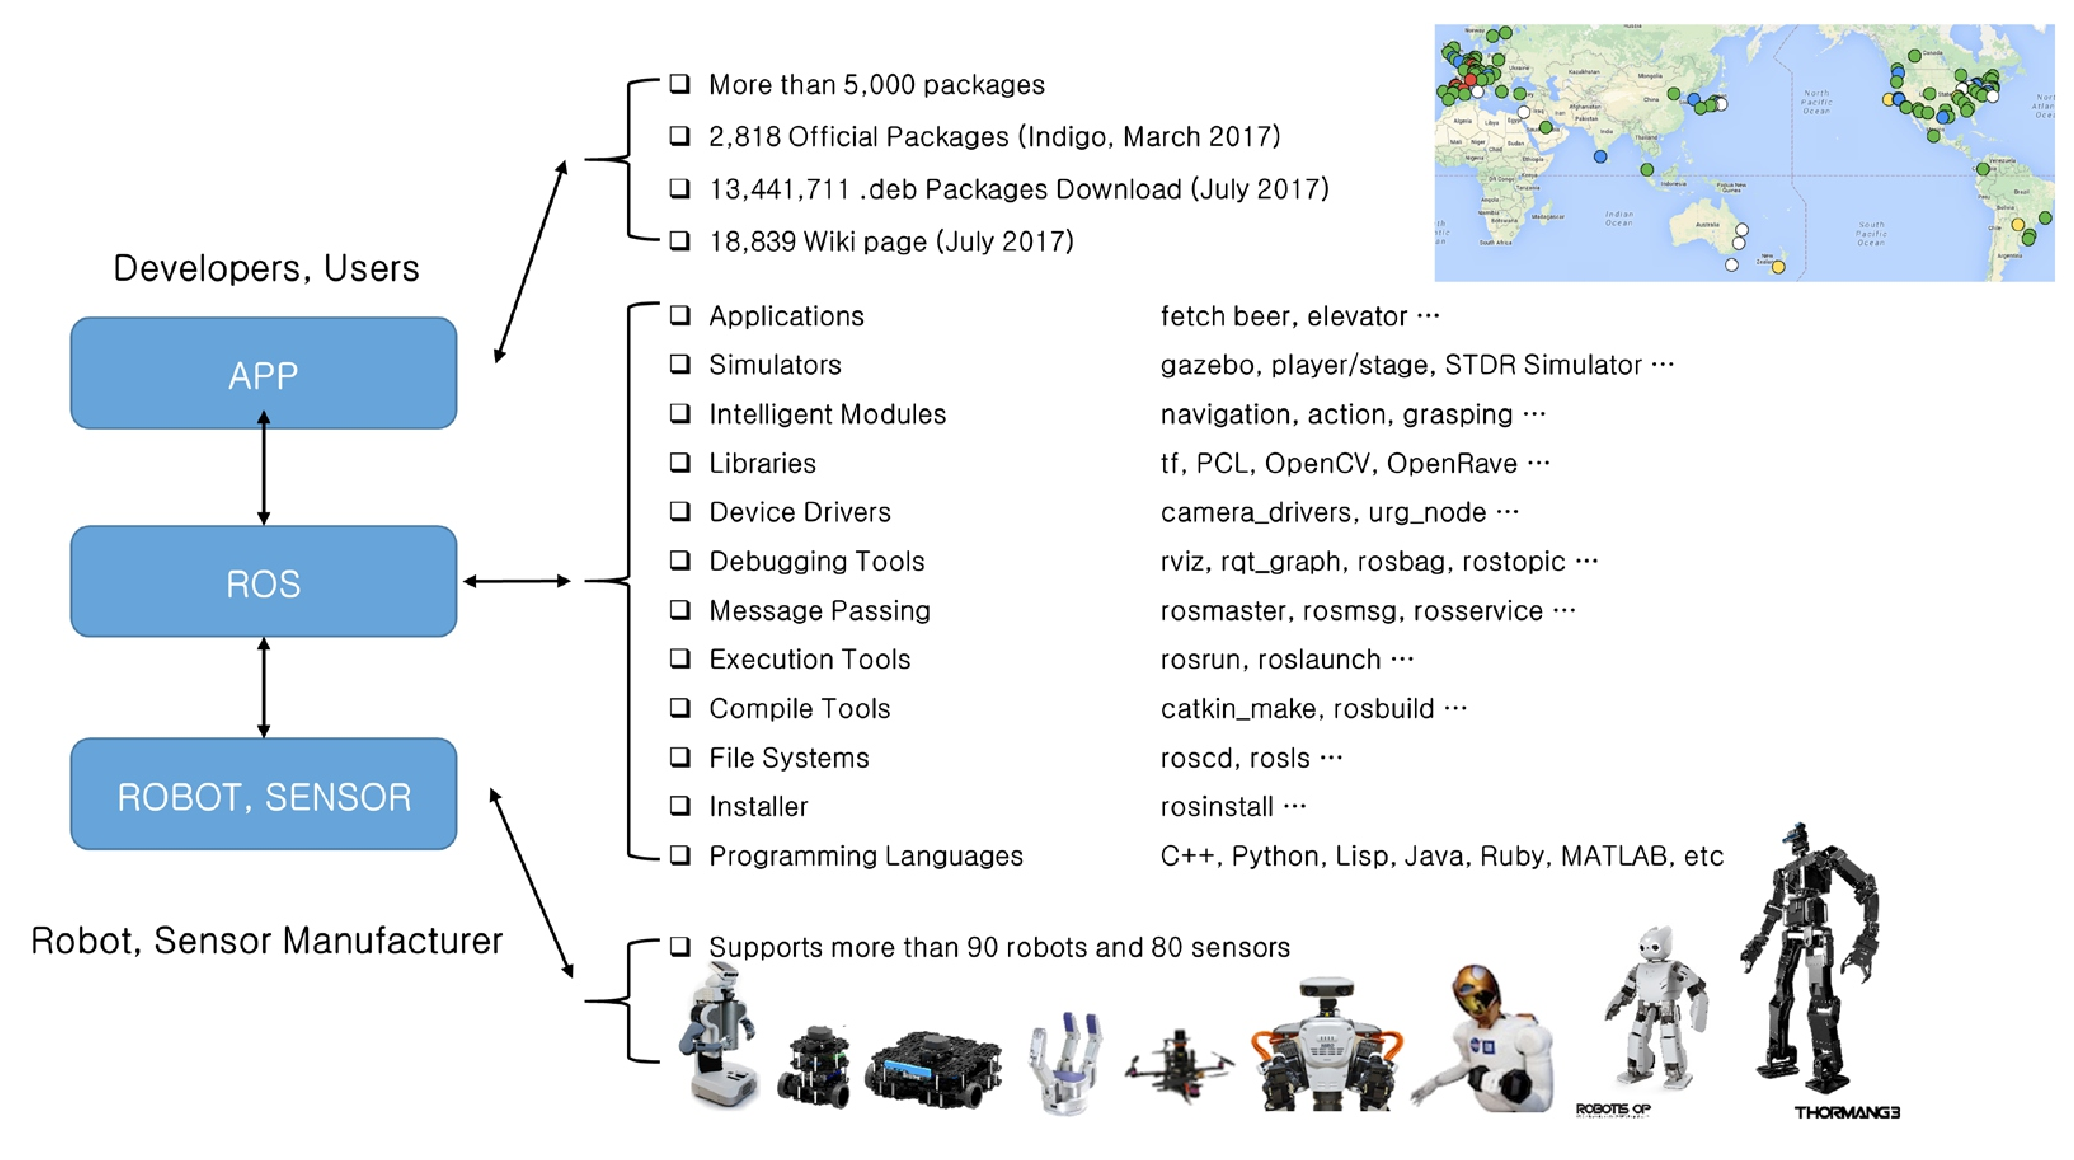
\includegraphics[width=1\linewidth]{chapter2/figs/Ecosystem.pdf}
	\caption{Hệ sinh thái ROS}
	\label{fig:Ecosystem}
\end{figure}
\section{Vấn đề SLAM và điều hướng robot}
\subsection{SLAM là gì?}
\begin{figure}[tph]
	\centering
	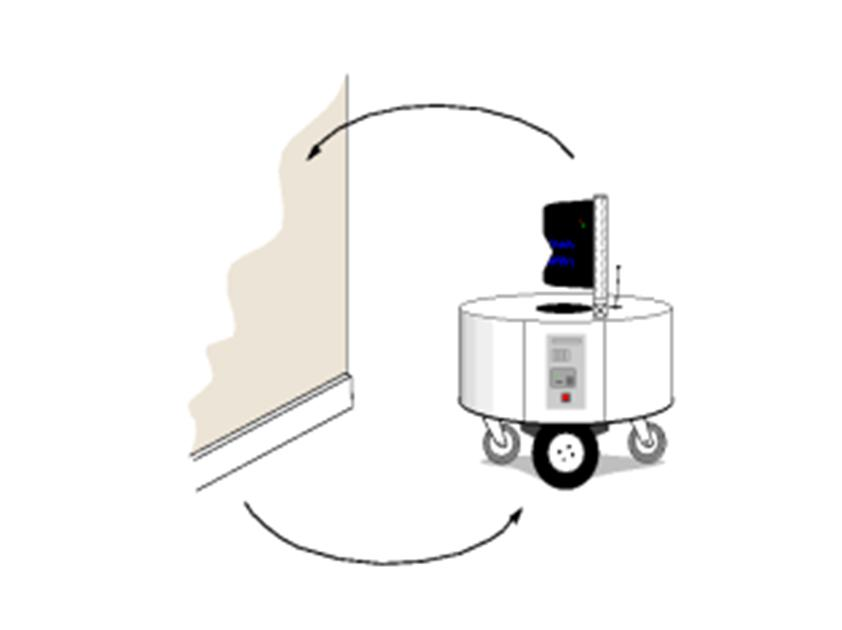
\includegraphics[width=0.7\linewidth]{chapter2/figs/slam}
	\caption{Khái niệm SLAM}
	\label{fig:slam}
\end{figure}
SLAM (Simultaneous Localization And Mapping) là đồng thời ước tính vị trí và xây dựng bản đồ trong môi trường chưa biết. Đây là công nghệ cốt lõi cho điều hướng robot cũng như điều khiển robot tự hành.

Các encoder và IMU thường được sử dụng để ước tính vị trí (bài toán odometry). Encoder tính toán xấp xỉ vị trí của robot bằng phương pháp tính dead reckoning với việc đo số vòng quay của hai bánh lái. Quá trình này xuất hiện sai số so với thực tế đo được bằng IMU. 

Vị trí ước tính này có thể được hiệu chỉnh một lần nữa  thông qua thông tin từ môi trường xung quanh bằng các cảm biến khoảng cách hoặc camera được dùng để tạo bản đồ. Các phương pháp ước tính vị trí như Kalman Filter, Markov localization...

Các cảm biến khoảng cách như cảm biến siêu âm, cảm biến hồng ngoại, cảm biến laser cũng thường được dùng cho việc tạo bản đồ. Ngoài ra, các camera cũng được sử dụng để đo khoảng cách như stereo camera, hoặc cũng có thể sử dụng các camera thông thường cho bài toán visual SLAM.

Một vài phương pháp định vị cho robot như:
\begin{itemize}
	\item Kalman Filter
	\item Particle Filter
\end{itemize}

SLAM là một bài toán khó trong robotics vì muốn định vị tốt thì phải có được bản đồ môi trường xung quanh nó và muốn có bản đồ chính xác thì phải định vị tốt. Đây là bài toán \textbf{"con gà - quả trứng"} (\figurename{\ref{fig:slam}}). Hơn nữa, các thông tin mà robot có được từ định vị, từ cảm nhận môi trường đều là các thông tin tương đối.

\subsection{Ứng dụng SLAM trong robot}
Các thuật toán như gmapping, cartographer và rtapmap thường được sử dụng cho bài toán SLAM, tuy nhiên, em lựa chọn thuật toán gmapping cho bài toán SLAM trong luận văn này. 

Các thành phần phần cứng của hệ thống phục vụ cho bài toán SLAM:
\begin{itemize}
	\item Nền tảng robot di động hai bánh chủ động, di chuyển trên mặt phẳng X-Y
	\item Encoder và IMU được sử dụng để ước tính trạng thái robot
	\item Sử dụng các cảm biến khoảng cách và Lidar.
\end{itemize}
\begin{figure}[tph]
	\centering
	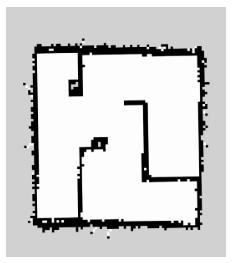
\includegraphics[width=0.4\linewidth]{chapter2/figs/OGM}
	\caption{Occupancy Grid Map}
	\label{fig:ogm}
\end{figure}

\textbf{Tạo bản đồ}: Ở đây sử dụng bản đồ 2 chiều Occupancy Grid Map (OGM)
 (\figurename{\ref{fig:ogm}}). Với sự thể hiện màu trắng là nơi robot có thể di chuyển được, màu đen là vùng bị chiếm dụng và robot không thể di chuyển. Màu xám là khu vực chưa biết. 
 
 Các khu vực trên bản đồ được thể hiện bằng giá trị của ảnh gray với giá trị từ '0' tới '255'. Các giá trị này thể hiện xác suất  chiếm dụng, được tính bởi phương pháp Bayes. 
 
 Quá trình tạo bản đồ sẽ lưu trong file '.pgm' và '.yaml' chứa các thông tin bản đồ,
 \begin{lstlisting}[numbers=none]
image: map.pgm 
resolution: 0.050000
origin: [-10.000000, -10.000000, 0.000000] 
negate: 0
occupied\_thresh: 0.65 
free\_thresh: 0.196
 \end{lstlisting}
 
\textbf{Thông tin yêu cầu cho SLAM}\\
\begin{figure}[tph]
	\centering
	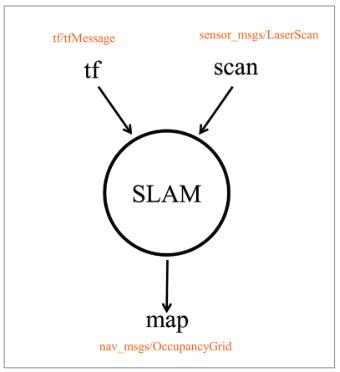
\includegraphics[width=0.5\linewidth]{chapter2/figs/slam_requiredInfo}
	\caption{Thông tin yêu cầu cho SLAM}
	\label{fig:slamrequiredinfo}
\end{figure}
Quá trình SLAM cần có thông tin sự dịch chuyển của robot được gọi là 'tf' (transform) và thông tin mà Lidar quét được trong 'scan' (\figurename{\ref{fig:slamrequiredinfo}}).

\textbf{Quá trình SLAM}:\\
\begin{figure}[tph]
	\centering
	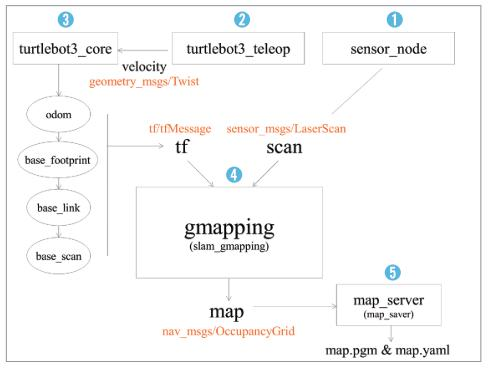
\includegraphics[width=0.7\linewidth]{chapter2/figs/slam_flowChart}
	\caption{Quá trình SLAM}
	\label{fig:slamflowchart}
\end{figure}

Quá trình tạo bản đồ với SLAM được mô tả như trong \figurename{\ref{fig:slamflowchart}}.

\subsection{Điều hướng robot}
\begin{figure}[tph]
	\centering
	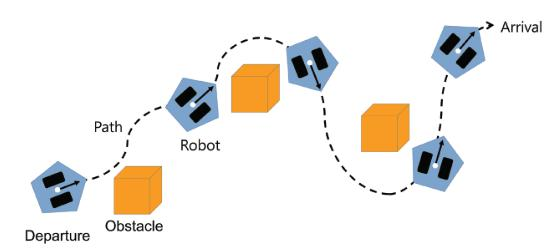
\includegraphics[width=0.7\linewidth]{chapter2/figs/navigation}
	\caption{Điều hướng robot}
	\label{fig:navigation}
\end{figure}
Điều hướng robot là bài toán điều khiển robot tới một vị trí xác định, nó không thực sự dễ đối với robot. Điều quan trọng là robot phải biết được bản đồ của môi trường và tự định vị được nó đang ở đâu trong bản đồ ấy. Bài toán tìm và tối ưu quỹ đạo di chuyển giữa rất nhiều quỹ đạo, và tránh vật cản cũng như các vật dụng cũng rất quan trọng, và không phải là một nhiệm vụ dễ dàng (\figurename{\ref{fig:navigation}})

Trình tự thực hiện như sau:
\begin{itemize}
	\item \textbf{Cảm nhận - sensing}
	Trên bản đồ, robot cập nhật dữ liệu từ encoder, cảm biến IMU, và đo khoảng cách từ LIDAR đến xung quanh
	\item \textbf{Định vị - localization/pose estimation}
	Dựa trên dữ liệu từ encoder, IMU và LIDAR, công đoạn ước tính vị trí robot được thực hiện trên bản đồ có sẵn. Sử dụng AMCL.
	\item \textbf{Tính quỹ đạo di chuyển - motion planning}
	Tạo quỹ đạo từ vị trí hiện tại đến đích, quỹ đạo bao gồm quỹ đạo tổng thể trên bản đồ và quỹ đạo local nhỏ hơn xung quanh robot
	Di chuyển tránh vật cản - Move/Obstacle Avoidance
	\item \textbf{Tránh vật cản}
	Sau khi quỹ đạo được đưa ra, robot di chuyển dựa trên quỹ đạo đó. Bởi quá trình cảm nhận, định vị và tính quỹ đạo di chuyển liên tục được cập nhật trong lúc robot di chuyển, các vật cản hoặc vật thể chuyển động đột nhiên xuất hiện sẽ được tránh bởi thuật toán DWA.
		
\end{itemize}

\subsection{Một số cơ sở lý thuyết}
\textbf{Localization Methodology -  Ước tính trạng thái robot bằng Particle Filter }\\
Particle Filter là  một kỹ thuật để dựa đoán thông  qua mô phỏng dựa trên phương pháp try-and-error.  

Trong  pp  này,  vị thế ban đầu robot được mô tả  bởi rất nhiều các điểm gọi là mẫu.  Ta  di chuyển các điểm này  đến  một vị trí và hướng mới  dựa trên mô hình  chuyển động và xác suất của  robot,  đồng thời đo  lường  tỉ lệ  của  mỗi điểm dựa theo  giá  trị thực  đo được,  cùng lúc giảm dần  độ sai  số đến vị trí  chính xác.  Đối với mobile robot,  mỗi điểm được mô tả dưới dạng:
a  particle =  pose (x,y,I), weight

Mỗi  điểm là một điểm  ảo nhỏ  thể hiện vị trí và hướng ước  tính  thể hiện bởi x,y  và  i  và phần trăm khả năng  của mỗi điểm.

Chu trình  lọc điểm chạy theo 5  bước, ngoài bước 1  là khởi tạo,  từ bước 2  đến 5  sẽ liên tục lặp lại để ước tính vị trí robot.  Nói theo cách khác,  đây là phương pháp để ước  tính vị trí robot  bằng liên tục cập nhật mô hình phân bố các điểm  thể  hiện xác suất  vị  trí robot  trong mặt phẳng.
\begin{enumerate}
	\item \textbf{Khởi tạo  -  Initialization}:
	Bởi vị trí và hướng ban đầu  robot là  chưa biết,  các điểm được sắp xếp ngẫu nhiên trong khu vực  mà ở đó vị  trí và hướng robot có khả năng là đúng,  ta có N  điểm.  Mỗi điểm  có  phần trăm đúng là 1/N,  và  tổng  khả năng là  1.  Nếu vị trí ban đầu được cho trước,  các  điểm này sẽ đặt gần robot.
	\item \textbf{Dự đoán -  prediction}:
	Khi robot di chuyển,  cùng lúc  các dữ liệu đo lường từ cảm  biến,  các điểm dự đoán cũng di chuyển theo
	\item \textbf{Cập nhật -  update}:
	Dựa trên  dữ liệu từ cảm biến,  xác suất của mỗi điểm được  tính và phần trăm khả năng đúng được cập nhật theo.
	\item \textbf{Dự đoán  vị trí và  hướng - pose estimation}:
	Vị trí,  hướng và  phần trăm khả năng  của  tất cả  các điểm được dùng để tính các  gía trị trung bình và lớn  nhất cho việc ước tính vị trí robot
	\item \textbf{Lấy lại mẫu  -  resampling}:
	Bước này sẽ loại bỏ những điểm có khả năng  chính xác thấp  để tạo những  điểm mới  chính xác hơn. Số lượng N  điểm phải được giữ nguyên
\end{enumerate}

Lấy  số lượng điểm mẫu là đủ,  bộ lọc  điểm có thể chính xác hơn so với bộ lọc Kalman.  Tuy nhiên nếu  số lượng không đủ,  phương pháp này  sẽ không chính xác.  SLAM dựa trên  Bộ lọc điểm Rao-Blackwelled (RBPF)  tối ưu cả lọc điểm và lọc Kalman  cùng  lúc,  nó cũng  được ứng dụng rộng rãi trong  
cách tiếp cận các vấn đề SLAM.  

\textbf{Costmap}\\
\begin{figure}[tph]
	\centering
	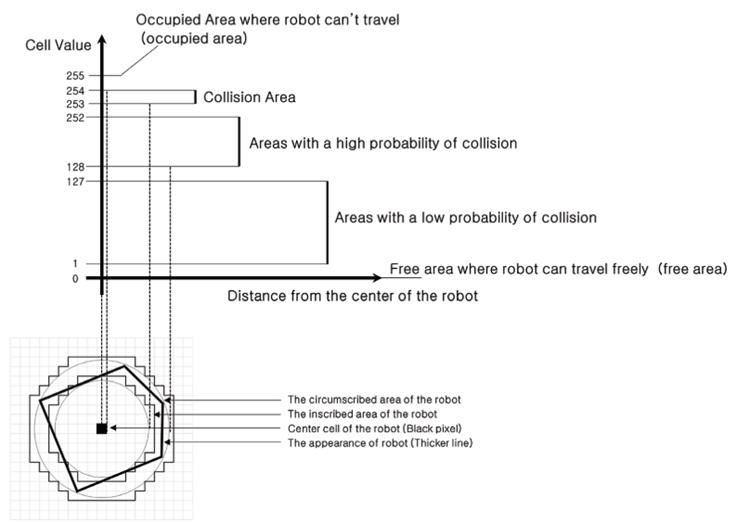
\includegraphics[width=0.7\linewidth]{chapter2/figs/costmap}
	\caption{Mối quan hệ giữa vật cản và giá trị costmap}
	\label{fig:costmap}
\end{figure}
\begin{figure}[tph]
	\centering
	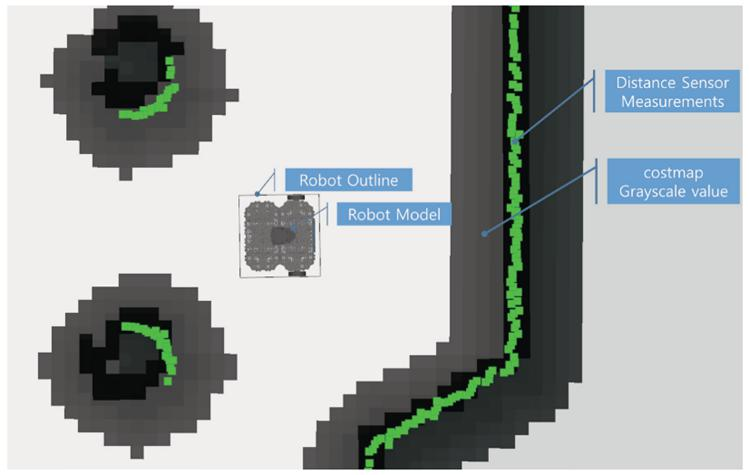
\includegraphics[width=0.7\linewidth]{chapter2/figs/costmap1}
	\caption{Sự thể hiện costmap}
	\label{fig:costmap1}
\end{figure}
\begin{itemize}
	\item Vị trí robot được ước tính thông qua encoder và IMU. Khoảng cách robot đến môi trường xung quanh thu được từ LIDAR. Vị trí robot và sensor, thông tin về vật cản, bản đồ lưới coi như là kết quả của SLAM và được dùng để tải stastic map có sẵn và làm rõ các khu vực có đồ vật, khu vực đi được và khu vực chưa biết.
	\item Costmap tính toán khu vực có vật cản, khu vực có thể xảy ra va chạm, và khu vực robot di chuyển an toàn. Dựa trên loại định hướng, costmap được chia thành 2 loại. 'Global\_costmap' lên quỹ đạo tổng thể trên bản đồ cố định cho trước.
	\item 'Local\_costmap' cũng là lên quỹ đạo nhưng trong khu vực mà robot nhìn thấy được, xung quanh robot. Mặc dù mục đích 2 loại costmap trên là khác nhau, nhưng chúng đều được hiển thị giống nhau.
	\item Costmap thể hiện đặc tính của các mắt lưới trên bản đồ theo vùng giá trị 0-255 (\figurename{\ref{fig:costmap}})
\end{itemize}

\textbf{AMCL}\\
\begin{itemize}
	\item Mục đích cuối cùng của MCL pose estimation là xác định robot ở đâu trên môi trường đã biết. Vậy nên ta cần biết (x,y) và hướng (theta). Vì thế nên MCL sẽ tính toán xác suất vị trí robot, không có 1 giá trị chính xác.
	\item Đầu tiên, vị trí và hướng (x,y, theta) tại thời điểm t được ký hiệu là $x_p$.
	\item Dữ liệu khoảng cách quét tại thời điểm t được ký hiệu là $z_{0…t}={z_0,z_1,…, z_t}$
	\item Dữ liệu dịch chuyển lấy từ encoder tại t: $u_(0…t)={u_0,u_1, …, u_t}$
	\item Sau đó bắt đầu tính toán:
	\[{\rm{bel(}}{{\rm{x}}_{\rm{t}}}{\rm{)  =  p(}}{{\rm{x}}_{\rm{t}}}{\rm{|}}{{\rm{z}}_{{\rm{0}}...{\rm{t}}}}{\rm{, }}{{\rm{u}}_{{\rm{0}}..{\rm{t}}}}{\rm{)}}\]
	\item Ở bước dự đoán, vị trí robot $bel'({x_t})$ tại khung thời gian kế tiếp được tính bằng cách sử dụng motion model $p({x_t}|{x_{t - 1}},{u_{t - 1}})$ của robot, xác suất $bel({x_{t - 1}})$ tại vị trí trước đó và dữ liệu di chuyển u nhận được từ encoder:
	$$Be{l^\prime }\left( {{x_t}} \right) = \int p\left( {{x_t}|{x_{t - 1}},{u_{t - 1}}} \right)bel\left( {{x_{t - 1}}} \right)d{x_{t - 1}}$$
	\item Bước tiếp theo là cập nhật. Lúc này, mô hình cảm biến $p(z_t |x_t)$, xác suất $bel(x_t)$ và hằng số chuẩn hóa eta $({\eta _t})$ được dùng để có xác suất chính xác hơn $Bel\left( {{x_t}} \right) = {{\rm{\eta }}_t}p\left( {{z_t}|{x_t}} \right)bel\prime \left( {{x_t}} \right)$
	\item Tiếp theo là ước tính vị trí bằng cách tạo ra N điểm bằng phương pháp lọc điểm sử dụng xác suất tính toán $bel'({x_t})$ của vị trí hiện tại. Trong MCL, từ "sample - mẫu" thay thế cho "particle - điểm" và xử lý qua SIR (Sampling Importance weighting Re-sampling). Bước đầu tiên là xử lý mẫu (sampling process). Ở đây một tập hợp mẫu mới xt được triết xuất thông qua mô hình chuyển động $p({x_t}|{x_{t - 1}},{u_{t - 1}})$  tại xác suất $bel({x_{t - 1}})$ của vị trí trước đó. Mẫu "i" $xt(i)$ trong tập hợp mẫu xt, dữ liệu khoảng cách zt, và hằng số chuẩn hóa .... Được dùng  để tính trọng số ....
	$\omega _t^{\left( i \right)} = {\rm{\eta }}p({z_t}|x_t^{\prime \left( i \right)})$
	\item Cuối cùng là quá trình làm mới mẫu, tạo ra N mẫu mới của tập hợp Xt sử dụng mẫu cũ xt và trọng số vừa tính:
	\[{X_t} = \left\{ {x_t^{\left( j \right)}{\rm{|}}j = 1 \ldots N} \right\} \sim \left\{ {x_t^{\prime \left( i \right)},\omega _t^{\left( i \right)}} \right\}\]
	Bằng cách lặp lại quá trình SIR trên trong khi di chuyển, vị trí ước tính robot tăng dần độ chính xác
\end{itemize}

\textbf{Dynamic Window Approach (DWA)}\\
\begin{figure}[tph]
	\centering
	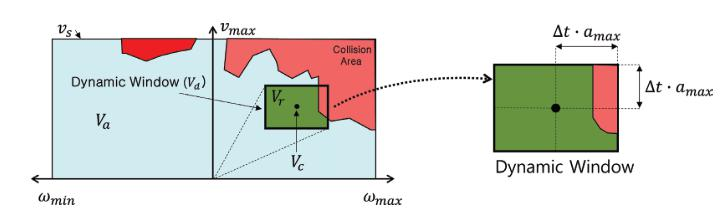
\includegraphics[width=0.8\linewidth]{chapter2/figs/dwa}
	\caption{Không gian tìm kiếm vận tốc và cửa sổ động của robot}
	\label{fig:dwa}
\end{figure}
\begin{figure}[tph]
	\centering
	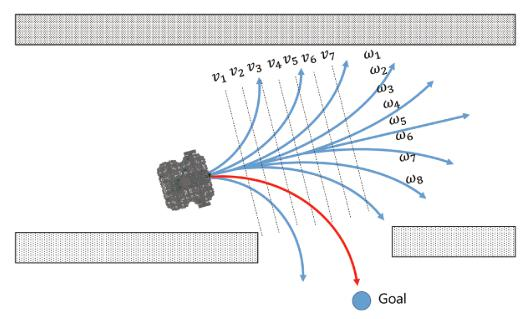
\includegraphics[width=0.7\linewidth]{chapter2/figs/dwa1}
	\caption{Phép dịch chuyển vận tốc dài và vận tốc góc}
	\label{fig:dwa1}
\end{figure}

\begin{itemize}
	\item Đây là  1 phương pháp phổ biến trong việc lên quỹ đạo tránh vật cản và tránh vật cản. Phương pháp này lựa chọn 1 tốc độ mà có thể nhanh chóng tiến đến điểm đích và tránh vật cản mà có thể có khả năng cao va chạm với robot. Trong ROS, Trajectory Planner (bộ phận lên quỹ đạo) được dùng cho lên quỹ đạo local, nhưng DWA đang được ứng dụng nhiều bởi tính năng vượt trội của nó. 
	\item Đầu tiên, robot không ở trong hệ tọa độ x-y, nhưng ở trong không gian tìm kiếm tốc độ (velocity search space) với vận tốc thẳng v và vận tốc quay omega. Trong không gian này, robot có tốc độ cho phép tối đa dựa trên giới hạn phần cứng, đây được gọi là Dynamic Window.
\end{itemize}
